\defi{7.1} Sea $C$ un punto de $\P$ y $k > 0$. Una \textbf{homotecia} $\eta_{C,k}:\P \rightarrow \P$ es una aplicación tal que a cada punto $P \in r_{CP}$ le hace corresponder un punto $\eta_{C,k}(P) \in r_{CP}$ tal que $C\eta_{C,k}(P) = kCP$. $k$ es la \textbf{razón de homotecia}.

\obs{7.2} Sea $X \in \P$, $\eta_{C,k}$ y $\gamma$ una aplicación del \axioma{P3}. Entonces se cumple que $\gamma(\eta_{C,k}(X)) = \gamma(C) + k(\gamma(X)-\gamma(C))$

\obs{7.3} Toda homotecia es una biyección que tiene
\begin{itemizex}
	\item Identidad: $\eta_{C,1}$
	\item Inversa: $\eta_{C,1/k}$
\end{itemizex}

\tma{7.4}/\cor{7.5} Sean $A, B$ y $\eta_{C,k}$, entonces $\eta_{C,k}(A)\eta_{C,k}(B) = kAB$. Además, $\eta_{C,k}[A,B] = [\eta_{C,k}(A), \eta_{C,k}(B)]$.

\obligatorio\dem{7.4 Suponemos $A,B,C$ no alineados. Por definición, $C,A, \eta_{C,k}(A)$ están alineados, y lo mismo con $C,B,\eta_{C,k}(B)$. Los triángulos $\triangle ABC$ y $\triangle \eta_{C,k}(A)\eta_{C,k}(B)C$ comparten $\angle C$.
Por el \tma{del coseno} aplicado a $\angle C$:
$$AB^2 = AC^2+BC^2-2BC\cdot AC\cos(\angle C)$$
Por otra parte:
$$\eta_{C,k}(A)\eta_{C,k}(B)^2 = \eta_{C,k}(A)C^2+\eta_{C,k}(B)C^2$$$$-2\eta_{C,k}(A)C\cdot\eta_{C,k}(B)C\cos(\angle C)$$
Por definición $\eta_{C,k}(A)C=kAC$ y $\eta_{C,k}(B)C=kBC$, luego
$$\eta_{C,k}(A)\eta_{C,k}(B)^2 = k^2AC^2+k^2AC^2-2k^2AC^2BC^2\cos(\angle C) = $$
$$k^2( AC^2+BC^2-2BC\cdot AC\cos(\angle C)) = k^2AB^2$$
Luego $\eta_{C,k}(A)\eta_{C,k}(B) = kAB$}

\obligatorio\dem{7.5 Si $X\in[A,B]$ entonces $AX+XB = AB$. Por tanto:
$$kAX+kXB = kAB \iff $$$$ \eta_{C,k}(A)\eta_{C,k}(X)+\eta_{C,k}(X)\eta_{C,k}(B)=\eta_{C,k}(A)\eta_{C,k}(B)\iff$$$$\eta_{C,k}(X)\in [\eta_{C,k}(A),\eta_{C,k}(B)]$$}
\tma{7.7} Toda homotecia envía un ángulo a un ángulo congruente, y toda recta a una paralela.

\defi{7.8} Una \textbf{semejanza} es una combinación de homotecias e isometrías.

\cor{7.10/7.11} / \tma{7.19} Toda semejanza envía rectas a rectas, segmentos a segmentos, y conserva los ángulos. Toda biyección $\psi$ que cumpla estas condiciones es una semejanza.

\tma{7.12} / \cor{7.13} Toda semejanza $\delta$ cumple que $\delta(A)\delta(B) = kAB$, donde $k$ es la razón de semejanza. Dados $A,B,C,D$, entonces se cumple que 
$$\frac{AB}{CD} = \frac{\delta(A)\delta(B)}{\delta(C)\delta(D)}$$
\obligatorio \dem{$$\frac{\delta(A)\delta(B)}{\delta(C)\delta(D)} = \frac{kAB}{kCD} = \frac{AB}{CD}$$}

\tma{7.15} Si $\angle A = \angle B$, entonces existe $\delta$ tal que $\delta(\angle A) = \angle B$.

\tma{7.18} Sean $\triangle ABC$ y $\triangle AB'C'$ que comparten $\angle A$ y $A,B,B'$ están alineados, así como $A, C, C'$. Entonces si existe $k$ tal que $AB' = kAB$ y $AC' = kAC$ entonces $\triangle ABC$ y $\triangle AB'C'$ son semejantes, $r_{BC} \parallel r_{B'C'}$ y $B'C' = kBC$.

\defi{7.20} Se llama \textbf{mediana} al segmento que une cada vértice con el punto medio del lado opuesto de un triángulo. Es decir, dado $\triangle ABC$, las medianas son $[A, \m[B,C]]$, $[B, \m[A,C]]$ y $[C, \m[A,B]]$.

\tma{7.21} Las tres medianas de un triángulo cortan en un punto $G$, llamado \textbf{baricentro}.
\begin{figure}[H]
	\centering
	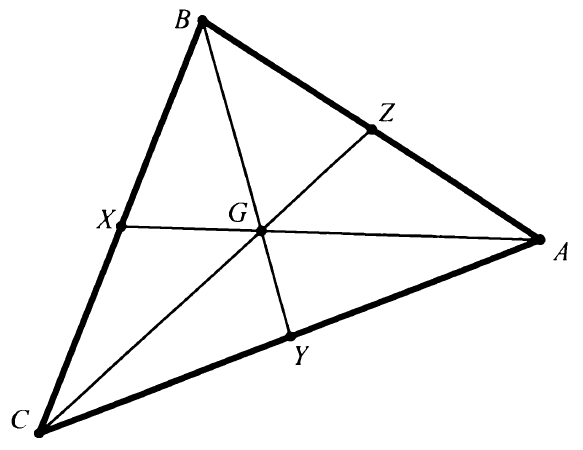
\includegraphics[width=5.5cm]{figuras/7-21.png}
	\vspace{-1em}
\end{figure}
\obligatorio\dem{Definimos $X = \m[B,C], Y = \m[A,C], Z = \m[A,B]$ y sea $G$ $[B,Y] \cap [C,Z]$. El punto existe porque, si definimos la recta $r_{BY}$, entonces $C$ está en uno de los semiplanos de la recta (pongamos, $H^2$) y, si $A \in H^1$, entonces $Z \in H^1$, $C$ y $Z$ están en distintos semiplanos de $r_BC$.
Si tomamos $\triangle ABC$ y $\triangle AZY$ entonces, por ser $Y,Z$ puntos medios, entonces, por el \tma{7.18}, $r_{YZ} \parallel r_{BC}$ y $BC = 2YZ$. Además, por ser los ángulos entre $[C,Z]$ y $[B,Y]$ alternos internos, los triángulos $\triangle GYZ$ y $\triangle GBC$ son semejantes de razón $2$. Por tanto, $GB = 2GY$ y $GC = 2GZ$.
Si repetimos esto con $[A,X]$ y $[B,Y]$, entonces existe un punto $G'$ tal que $G'A = 2G'X$ y $G'B = 2G'Y$. Como $\frac{G'B}{G'Y} = \frac{GB}{GY}$, entonces $G = G'$ y las tres medianas cortan en $G$. }

\tma{7.23} Las tres mediatrices de un tríangulo cortan en un punto, el \textbf{circuncentro}.
\begin{figure}[H]
	\centering
	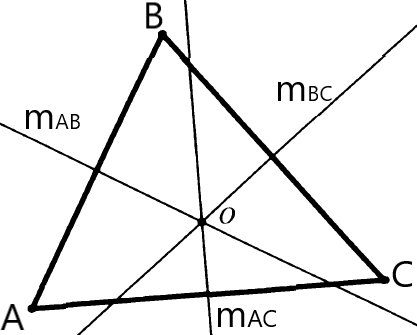
\includegraphics[width=4.5cm]{figuras/7-23.png}
	\vspace{-1em}
\end{figure}
\obligatorio\dem{Si $\triangle ABC$ es un triángulo, las mediatrices $m_{AB}$ y $m_{BC}$ cortan en un punto $O$. Si no cortaran, entonces $m_{AB} \parallel m_{BC}$, y como $r_{AB}\perp m_{AB}$ y $m_{BC} \perp r_{BC}$ entonces $r_{AB} \parallel r_{BC}$, lo cual es absurdo. Por ser $m_{BC}$ mediatriz, entonces $OB = OC$, y $OA = OB$ para $m_{AB}$. Entonces $OA = OC$ y por tanto $O \in m_{AC}$, luego $O$ corta las tres mediatrices.  }

\tma{7.24} Las tres alturas de un triángulo se cortan en el \textbf{ortocentro}
\begin{figure}[H]
	\centering
	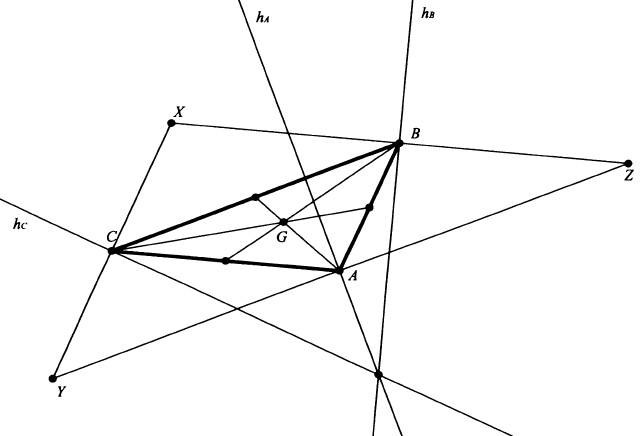
\includegraphics[width=8.5cm]{figuras/7-24.png}
	\vspace{-1em}
\end{figure}
\obligatorio\dem{Sea $\triangle ABC$ el triángulo con baricentro $G$ y sean $h_A, h_B, h_C$ sus alturas. Consideramos la semejanza $\tau = \sigma_G \eta_{G,2}$, de modo que $\triangle ABC$ se transforma en $\triangle XYZ$, con $\tau(A) = X, \tau(B) = Y, \tau(C) = Z$. Por las propiedades de las semejanzas, $r_{BC} \parallel r_{YZ}, r_{AC} = r_{XZ}, r_{AB} \parallel r_{XY}$, y se cumple que $A = \m[Y,Z], B=\m[X,Z], C = \m[X,Y]$. Por tanto, ahora $h_A = m_{YZ}, h_B = m_{XZ}, h_C = m_{XY}$ y, por tanto, el ortocentro de $\triangle ABC$ es el circuncentro de $\triangle XYZ$.}

\tma{7.25 [Recta de Euler]} 
Dado un triángulo, su baricentro $G$, ortocentro $O$ y circuncentro $H$ pertenecen a una misma recta (si el triángulo no es equilátero). Además, $OH = 2OG$.

\obligatorio\dem{Si partimos del triánguo con baricentro $G$ y aplicamos la semejanza $\tau = \sigma_G\eta_{G,2}$, como en el \tma{7.24}, entonces se cumple que $\tau(O) = H$. Por ser $\sigma_G$, entonces $H\in r_{OG}$ y por ser $\eta_{G,2}$, entonces $OH = 2OG$.}

\cor{7.26} El \textbf{incentro} del triángulo es el punto donde se cortan las tres bisectrices del triángulo.

\ej{7.7 [Teorema de Ceva]} En $\triangle ABC$ sean $X \in [B,C], Y \in [C,A], Z \in [A,B]$. Si $X,Y,Z$ no coinciden con ninguno de los vértices del triángulo, entonces los segmentos $[A,X],[B,Y],[C,Z]$ se cortan en un punto sii
$$\frac{AZ}{ZB}\frac{BX}{XC}\frac{CY}{YA} = 1$$

\ej{7.8 [Teorema de Menelao]} Sea $\triangle ABC$ y sean $X \in r_{BC}, Y \in r_{CA}, Z \in r_{AB}$. Entonces, sii $X,Y,Z$ están alineados se cumple que 
$$\frac{AZ}{ZB}\frac{BX}{XC}\frac{CY}{YA} = 1$$








